
%----------------------------------------------------------------------------------------
%	PACKAGES AND THEMES
%----------------------------------------------------------------------------------------

\documentclass{beamer}

\usetheme{Warsaw}

\usepackage{listings}
\usepackage[utf8]{inputenc}
\usepackage{url}
\setbeamertemplate{itemize item}[triangle]
%----------------------------------------------------------------------------------------
%	TITLE PAGE
%----------------------------------------------------------------------------------------

\title{Java Development - Tools} % The short title appears at the bottom of every slide, the full title is only on the title page

\author{Venkatesh} % Your name
\institute{WDC}
\date{\today} % Date, can be changed to a custom date

\begin{document}

\lstset{
    basicstyle=\ttfamily\footnotesize,
    breaklines=true
    breakatwhitespace=true,
    language=C++,
    columns=fullflexible,
    keepspaces=true,
    breaklines=true,
    tabsize=3, 
    showstringspaces=false,
    extendedchars=true
    inputencoding=utf8
}

\begin{frame}
\titlepage % Print the title page as the first slide
\end{frame}

\begin{frame}{Outline}

  \begin{enumerate}

   \item Maven       - build automation tool
   \item Checkstyle  - coding style       
   \item SpotBugs    - static analysis tool
   \item JUnit 5     - Unit Testing

  \end{enumerate}
\end{frame}


%----------------------------------------------------------------------------------------
%	PRESENTATION SLIDES
%----------------------------------------------------------------------------------------

%----------------------------------------------------------------------------------------

\begin{frame}[fragile]
\frametitle{Maven}

\begin{itemize}
\item An \texttt{XML} file describes the project being built, its dependencies
\item Maven is plugin-excution framework
    \begin{itemize}
        \item All work is done by plugins
    \end{itemize}
\item Dynamically downloads plug-ins from one or more repositories
\end{itemize}

\end{frame}

\begin{frame}[fragile]
\frametitle{Maven}

\begin{figure}[ht]
       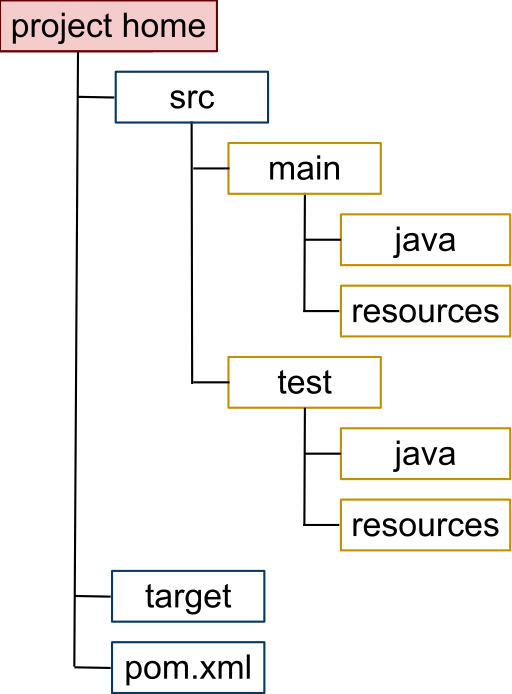
\includegraphics[width=5cm]{./images/Maven_CoC.png}
 \end{figure}
 
\end{frame}


\begin{frame}[fragile]
\frametitle{Maven Plugins}

A plugin provides a set of goals
\begin{block}{syntax for execution}
\begin{lstlisting}
    mvn [plugin-name]:[goal-name]
\end{lstlisting}
\end{block}

\begin{example}
 \begin{lstlisting}
mvn compiler:compile
\end{lstlisting}
\end{example}
\end{frame}


\begin{frame}[fragile]
\frametitle{Build lifecycle}

\begin{itemize}
\item validate
\item generate-sources
\item process-sources
\item generate-resources
\item process-resources
\item compile
\item process-test-sources
\item process-test-resources
\item test-compile
\item test
\item package
\item install
\item deploy
\end{itemize}


\end{frame}


\begin{frame}[fragile]
\frametitle{Example}


\end{frame}


\begin{frame}[fragile]
\frametitle{CheckStyle}

Checkstyle can examine
\begin{itemize}
\item \texttt{Javadoc} comments for classes, attributes and methods
\item Naming conventions of attributes and methods
\item Limit of the number of function parameters, line lengths
\item The spaces between some characters
\item ...
\end{itemize}

\end{frame}


\begin{frame}[fragile]
\frametitle{Maven Checkstyle plugin}
\begin{lstlisting}
      <plugin>
        <groupId>org.apache.maven.plugins</groupId>
        <artifactId>maven-checkstyle-plugin</artifactId>
        <version>3.0.0</version>

        <dependencies>
          <dependency>
            <groupId>com.puppycrawl.tools</groupId>
            <artifactId>checkstyle</artifactId>
            <version>8.11</version>
          </dependency>
        </dependencies>

\end{lstlisting}

\end{frame}

\begin{frame}[fragile]
\frametitle{Maven Checkstyle plugin...}
\begin{lstlisting}
        <executions>
          <execution>
            <id>validate</id>
            <phase>validate</phase>
            <configuration>
              <configLocation>google_checks.xml</configLocation>
              <encoding>UTF-8</encoding>
              <consoleOutput>true</consoleOutput>
              <failsOnError>true</failsOnError>
              <failOnViolation>true</failOnViolation>
              <violationSeverity>warning</violationSeverity>
            </configuration>
            <goals>
              <goal>check</goal>
            </goals>
          </execution>
        </executions>
      </plugin>
\end{lstlisting}
\end{frame}




\begin{frame}[fragile]
\frametitle{SpotBugs}

\begin{itemize}
\item SpotBugs is the successor of FindBugs
\item Static analysis tool to look for bugs in Java code
\item It checks for more than 400 bug patterns
\item \texttt{spotbugs-maven-plugin} can be added to pom.xml
\end{itemize}

\end{frame}


\begin{frame}[fragile]
\frametitle{Bug Descriptions}

\url{https://spotbugs.readthedocs.io/en/latest/bugDescriptions.html}


\end{frame}


\begin{frame}[fragile]
\frametitle{JUnit 5}

\begin{itemize}
\item Unit testing framework
\item \textit{JUnit 5} requires \textit{Java 8} (or higher) at runtime
\item \textit{JUnit 5} can be added to pom.xml
\end{itemize}

\end{frame}


\begin{frame}[fragile]
\frametitle{A first test case}

\begin{lstlisting}

import static org.junit.jupiter.api.Assertions.assertEquals;
import org.junit.jupiter.api.Test;

class FirstJUnit5Tests {

    @Test
    void myFirstTest() {
        assertEquals(2, 1 + 1);
    }

}
\end{lstlisting}
\end{frame}


\begin{frame}[fragile]
\frametitle{Annotations}

\begin{itemize}
\item \texttt{@Test}
\item \textit{@ParameterizedTest}
\item \textit{@RepeatedTest}
\item \texttt{@BeforeEach}
\item \texttt{@AfterEach}
\item \texttt{@BeforeAll}  : must be static methods
\item \texttt{@AfterAll}   : must be static methods
\item \texttt{@Disabled}
\end{itemize}

\end{frame}


\begin{frame}[fragile]
\frametitle{Test Classes and Methods}

\begin{block}{Test method}
method that is annotated with \texttt{@Test, @RepeatedTest, @ParameterizedTest, @TestFactory, or @TestTemplate}
\end{block}

\begin{block}{Test class}
any top level or static member class that contains at least one test method
\end{block}

\end{frame}


\begin{frame}[fragile]
\frametitle{Test Classes and Methods ...}

Methods annotated with 
\begin{itemize}
\item \texttt{@Test}
\item \texttt{@TestTemplate}
\item \texttt{@RepeatedTest}
\item \texttt{@BeforeAll}
\item \texttt{@AfterAll}
\item \texttt{@BeforeEach} or 
\item \texttt{@AfterEach} 
\end{itemize}
annotations \textit{must not return} a value

\end{frame}


\begin{frame}[fragile]
\frametitle{Example}


\end{frame}


\begin{frame}[fragile]
\frametitle{Assertions}

\begin{itemize}

\item assertions are \texttt{static} methods in the \texttt{org.junit.jupiter.api.Assertions} class

\end{itemize}
\end{frame}


\begin{frame}[fragile]
\frametitle{Example}


\end{frame}

\begin{frame}[fragile]
\frametitle{Repeated Tests}

\begin{itemize}
\item Repeat a test a specified number of times simply by annotating a method with \texttt{@RepeatedTest}

\end {itemize}

\begin{example}
 \begin{lstlisting}
@RepeatedTest(10)
void repeatedTest() {
    // ...
}
\end{lstlisting}
\end{example}

\end{frame}


\begin{frame}[fragile]
\frametitle{Parameterized Tests}

\begin{itemize}
\item Run a test multiple times with different arguments

\end {itemize}

\begin{example}
 \begin{lstlisting}
@ParameterizedTest
@ValueSource(strings = { "racecar", "radar", "121"})
void palindromesTest(String candidate) {
    assertTrue(isPalindrome(candidate));
}
\end{lstlisting}
\end{example}

\end{frame}



\begin{frame}[fragile]
\frametitle{Sources of Arguments}

\begin{itemize}
\item \texttt{@ValueSource}
    \begin{itemize}
    \item Used for providing a single parameter per parameterized test
    \end{itemize}
\item \texttt{@MethodSource}
    \begin{itemize}
            \item factory method, must be static 
            \item must return a \texttt{Stream, Iterable, Iterator}, or array of arguments
    \end{itemize}
\item \texttt{@CsvSource}

\end {itemize}

\end{frame}


\begin{frame}[fragile]
\frametitle{@ValueSource}
Following types of literal values are supported

\begin{itemize}
\item short
\item byte
\item int
\item long
\item float
\item double
\item char
\item java.lang.String
\item java.lang.Class
\end {itemize}
\end{frame}

\begin{frame}[fragile]
\frametitle{@ValueSource...}
\begin{example}
 \begin{lstlisting}
@ParameterizedTest
@ValueSource(ints = { 1, 2, 3 })
void testWithValueSource(int argument) {
    assertTrue(argument > 0 && argument < 4);
}
\end{lstlisting}
\end{example}
\end{frame}


\begin{frame}[fragile]
\frametitle{@MethodSource}
\begin{example}
 \begin{lstlisting}
@ParameterizedTest
@MethodSource("stringProvider")
void testWithSimpleMethodSource(String argument) {
    assertNotNull(argument);
}

static Stream<String> stringProvider() {
    return Stream.of("foo", "bar");
}
\end{lstlisting}
\end{example}
\end{frame}


\begin{frame}[fragile]
\frametitle{@CsvSource}

\begin{itemize}
\item Allows you to express argument lists as \textit{comma-separated} values
\end{itemize}

\begin{example}
 \begin{lstlisting}
@ParameterizedTest
@CsvSource({ "foo, 1", "bar, 2", "'baz, qux', 3" })
void testWithCsvSource(String first, int second) {
    assertNotNull(first);
    assertNotEquals(0, second);
}
\end{lstlisting}
\end{example}

\end{frame}


%------------------------------------------------
\begin{frame}
\frametitle{References}
\begin{thebibliography}{2} % Beamer does not support BibTeX so references must be inserted manually as below
\setbeamertemplate{bibliography item}[book]

\bibitem{Version 5.2.0} JUnit 5 User Guide
\bibitem{} \url{https://junit.org/junit5/docs/5.0.0-M2/api/org/junit/jupiter/api/Assertions.html}
\end{thebibliography}
\end{frame}

%------------------------------------------------

\begin{frame}
\Huge{\centerline{Thank You}}
\end{frame}


%----------------------------------------------------------------------------------------

\end{document} 

